\section{Literature Relevance and the Limits of Comparison}
\label{sec:evidence-distance}

\subsection{Basis for Classification}

We organize the literature by how the subject of each study relates to the target phase rather than by assigning whole papers to a single bin. One study may supply evidence separately on structure, on synthesis route, or on characterization method, and each conclusion applies only to the object that study actually observed. The literature falls into five classes: direct reports of the target compound; Zn-free members of the same tetragonal Ba--Y silicate family; structurally related compounds with a definite crystallographic relationship; synthesis studies usable as process references; and unrelated sources that cannot support any judgment about the target structure or recipe. The classification describes how far each conclusion reaches; it is not a judgment of paper quality.

\paragraph{Direct reports of the target compound.} The formula must match $\mathrm{Ba_5Y_{12}Zn[O(SiO_4)]_8}$, and the primary study must give both the preparation and the structure determination. At present only the open-system high-temperature solution growth and single-crystal X-ray study of Ababaikeri et al. qualifies~\cite{ababaikeri2024ba5y12zn}. It provides the sole direct experimental starting point, but it has not established an independently reproducible bulk phase-pure window.

\paragraph{Same-family tetragonal Ba--Y silicates.} These studies contain no Zn but bear directly on the historical nomenclature, the structural revision, or the phase-region relationships of the tetragonal Ba--Y silicates. Early work reported the tentative accompanying phase $\mathrm{Ba_{5+x}Y_{13}Si_8O_{41}}$~\cite{kolitsch2009crystal}; modern single-crystal work revised the related composition to a non-stoichiometric modulated structure~\cite{yamane2024synthesis}; and an independent study confirmed tetragonal $\mathrm{Ba_5Y_{13}[SiO_4]_8O_{8.5}}$ by several diffraction and compositional methods~\cite{gulay2024navigation}. These results constrain the historical formulas, the composition range, and the competing phases, but they are no substitute for reproducing the Zn-containing target phase.

\paragraph{Structurally related compounds, process references, and unrelated sources.} Ba--Zn--Si--O or Ba--Y--Si--O compounds with reliable crystallographic data can be used to compare polyhedral connectivity, cation sites, and the characterization of phase transitions~\cite{liu1993structures,lin1999phase,zou2021crystal,motozawa2022bay16si4o33}; studies that supply only a synthesis route, atmosphere, cooling program, or mechanical treatment can be used to decide what to record and how to characterize the products~\cite{redhammer2003beta,pang2005study,tzvetkov2001effects}. None of these sources lets the composition range of the target phase be inferred. Studies that offer nothing beyond elemental similarity, an application context, or general theoretical discussion, with no crystallographic or synthetic link, are left out of the condition comparison for the target phase~\cite{buerger1954the,erlebach2020thermomechanical,gu2025liba2gasi2o8}.

\begin{figure}[t]
  \centering
  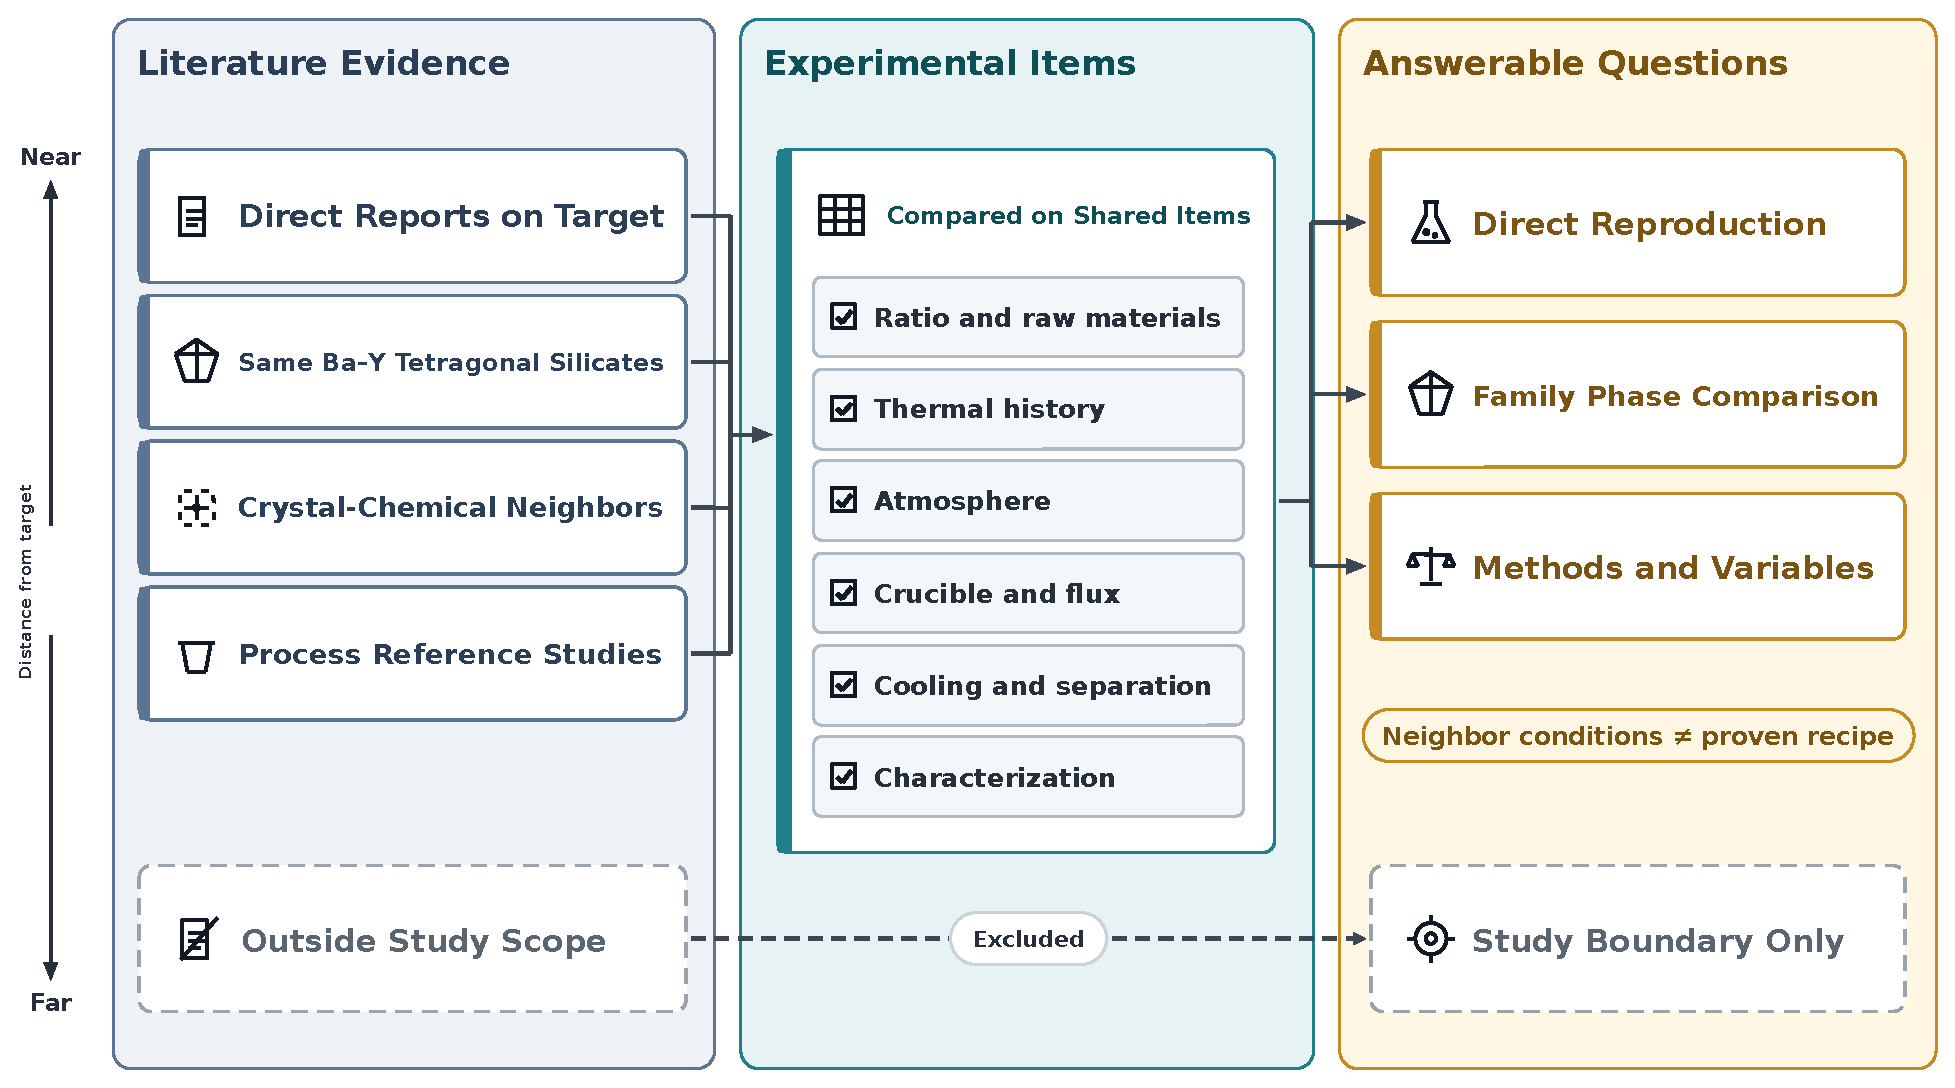
\includegraphics[width=\linewidth]{../figures/pdf/fig01_evidence_synthesis_map_en.pdf}
  \caption[What each class of literature can say about synthesizing the target compound]{\textbf{What each class of literature can say about synthesizing the target compound.} The left column lists, in order, direct reports of the target compound, same-family tetragonal Ba--Y silicates, structurally related compounds, process-reference studies, and unrelated sources; the middle column arranges starting materials, thermal history, atmosphere, container, cooling, and product characterization under the same experimental items; the right column states the questions each class can settle. Only one direct report of the target compound exists at present~\cite{ababaikeri2024ba5y12zn}. Values from related systems illustrate experimental variables and characterization methods only and cannot be taken as a verified recipe for the target phase.}
  \label{fig:evidence-map}
\end{figure}

Figure~\ref{fig:evidence-map} maps the subject of each publication to its experimental conditions and to the questions it can settle. A comparison first confirms which phase a publication actually studied and then sets starting materials, thermal history, atmosphere, container, and cooling conditions side by side under the same experimental items. This arrangement makes comparison easier but does not erase the structural differences between compounds. The more distant a publication is from the target phase, the more what can be borrowed shrinks to variable choices, experimental design, and characterization methods; specific temperatures, ratios, or flux amounts cannot be carried over directly.

\subsection{Structural Relatedness}

Structural relatedness requires, at a minimum, traceable crystallographic evidence; shared elements alone are not enough. Ba$M$SiO$_4$ ($M$~=~Co, Zn, Mg) has been assigned by single-crystal X-ray diffraction and powder neutron diffraction to the family of stuffed-tridymite derivatives~\cite{liu1993structures}. That result allows the tetrahedral networks of Zn, Mg, and Co to be compared, but the family contains no Y and belongs to a different structural series, so it is not direct evidence for the target phase. The low- and high-temperature forms of BaZn$_2$Si$_2$O$_7$ have been distinguished by neutron and X-ray diffraction~\cite{lin1999phase}; the monoclinic structure of Ba$_2$ZnSi$_2$O$_7$ was established by single-crystal refinement~\cite{kaiser2002crystal}; and diffraction on BaZnSi$_3$O$_8$ gave the connectivity network of its ZnO$_4$ and SiO$_4$ units~\cite{zou2021crystal}. These studies help define which structural parameters to compare, but they cannot say under which conditions the target phase can be reproduced.

The complexity of the four-coordinated Si networks in the Ba--Si--O system, and their response to temperature, serve only as an indirect structural reference~\cite{gorelova2016thermal}. The polymorphs of Y$_2$Si$_2$O$_7$ and their thermal-expansion data show that one composition can correspond to several structures, so comparisons spanning decades must check both the structural model and the observation temperature~\cite{dolan2008structures,becerro2004revision}. These results help frame the structural characterization questions, but they say nothing about the stability range of the target phase.

In short, same-family Ba--Y silicate studies can be used to test composition and phase region, structurally related studies to compare sites and characterization methods, and process-reference studies to sharpen experimental design. Specific synthesis conditions can be read only within the original object of study and its experimental range; they cannot be extrapolated simply because two compounds look ``similar''.

\subsection{What Counts as Unrelated}

Containing Ba and Si is not, by itself, structural relatedness. The structure refinement of benitoite-type BaSi$_4$O$_9$~\cite{finger1995refinement}, the trigonal structure of high-pressure BaSi$_4$O$_9$~\cite{hazen1999crystal}, the structure refinement of tribarium silicate~\cite{tillmanns1978refinement}, and the structure report on high-temperature Ba$_2$[Si$_4$O$_{10}$]~\cite{katscher1973the} all show that Ba--Si--O networks can adopt a range of structures, but none has the Y\slash Zn site correspondence the target phase requires. The report of 9R/6H perovskite-type structures in high-pressure Ba silicates further shows that a pressure route can lead to a different class of network altogether, from which the ambient-pressure route to the target cannot be inferred~\cite{yusa2007rhombohedral}.

Nor can a similar application context stand in for structural evidence. Optical studies of Ce$^{3+}$-doped Ba$_5$Si$_8$O$_{21}$ say nothing about the identity of the Y\slash Zn target phase~\cite{zhong2020combining}, and non-centrosymmetric LiBa$_2$GaSi$_2$O$_8$ resembles the target only in its optical application context, differing in both composition and structural series~\cite{gu2025liba2gasi2o8}. The classic concept of stuffed derivatives of the silica structures and the theory--experiment review of zero-thermal-expansion materials help to harmonize terminology and to understand thermomechanical behavior, but they cannot support recipe judgments for the target phase~\cite{buerger1954the,erlebach2020thermomechanical}.

Unrelated sources therefore serve only to mark the boundary of the study and do not enter the comparison of synthesis conditions for the target phase. Even where related sources appear in the same table, that placement means only that the experimental items are comparable, not that different compounds share a structure or phase-formation conditions.
